\chapter{Evaluation}
\label{chap:evaluation}
In this section, we will go over experiments done to evaluate our proposed approach. To evaluate the proposed approach, we built an event driven simulator that models the broadcast of transactions and blocks in the Bitcoin network. We decided to implement our own simulator because all the simulators that we found were either outdated or were not working~\footnote{Some examples \url{https://github.com/shadow/shadow-plugin-bitcoin} and \url{https://github.com/arthurgervais/Bitcoin-Simulator}}.

When evaluating our approach we took into consideration multiple metrics that we considered relevant for the changes we propose, we will now describe each one.
\begin{itemize}
	\item \textbf{Percentage of committed transactions} This metric is important because since we are effectively lowering the number of nodes that know of a transaction we wanted to make sure that in our approach transactions would not get lost in the dissemination process;
	\item \textbf{Commit time} This metric is also very susceptible to changes to the protocol especially changes like the ones we are proposing. Furthermore, making sure this metric does not cross critical values is also essential for our approach to be even considered one day to be integrated into the Bitcoin client;
	\item \textbf{Amount of messages sent} This metric is very important because it will determine if our approach brings anything of value to Bitcoin as this is the main metric we want to have an impact on by lowering it;
	\item \textbf{Amount of information sent} Similar to the previous metric but this one we did not expect to have a great impact as every transaction/block has to eventually be broadcast through the entire network.
\end{itemize}

\section{Simulator tuning}
\label{sec:sim_tuning}
To configure our simulator such that it reproduces faithfully the original protocol, we extended the \textsl{Bitcoin Core} client, the most used Bitcoin client to log metrics about the messages exchanged between clients. The metrics logged were the following: i) transactions advertisements; ii) received transactions; iii) transactions present in compact blocks that the node had to request to be able to rebuild the block. We deployed two instances of this client in two distinct physical locations for a whole month and used the metrics logged by these two clients to tune our simulator. Furthermore, we also used information publicly available on the website \url{https://blockchain.info/} to determine the number of transaction generated, the distribution of blocks generated by miners and the average transaction size. With all these metrics we implemented the original protocol, and then we added our changes to the protocol. We experimentally tuned our simulator so that the results observed were the same as the ones in the real client. The network model that we used in the experiments of Section~\ref{sec:sri} were composed solely of nodes that followed the protocol accordingly.

Due to the complexity of the protocol, simulating the full network resulted in resource intensive simulations that lasted for days.
%Running simulations of big Bitcoin networks in a language not optimised for efficiency resulted in the simulations being very demanding in terms of computations and space required which resulted in the simulations taking a long time (scale of days) to complete.
To overcome this, we scaled down the size of the simulated network a follows.
First,  we ran the original protocol with 6000 nodes and with 625 nodes and compared the metrics discussed beloq. The results we obtained were equivalent for both network sizes hence, for the rest of this section we consider a network size of 625 nodes. This proportional scaling between 6000 nodes (size registered when we started experimenting) and 625 nodes, allowed us to quickly explore different possible solutions and run multiple instances of each test. The results presented are an average of 3 independent runs that correspond to 34 hours in real time. We discarded the first and last 5 hours of each run in order to study the system in a stable state.


\section{Results}
\label{sec:results}

\subsection{Skewed Relay Impact}
\label{sec:sri}

We started by exploring the different possible solutions to reduce network usage without having a negative impact on the system. In all experiments below, we use the following notation: \textsl{Tn} where n specifies the value of the variable \textsl{max\_t\_nodes}; and \textsl{Rn} specifies the value of the variable \textsl{max\_r\_nodes} present in the previous algorithms. Note that for these experiments we did not used Algorithm~\ref{alg:inc} because we wanted to determine the best values for the aforementioned variables.

Initially we tested with multiple combinations of $n={1,2,3,4}$ for both \textsl{T} and \textsl{R}. After these preliminary experiments, we observed that for values of $n={3,4}$ the results were practically the same as the results without our approach. However, with $n={1,2}$ we observed a considerable reduction in the number of duplicated advertisements.
These results also support our logs in the real client, where the average number of duplicates was $6.6$. With this in mind, for the rest of the experiments, we considered only the combinations of: T2\_R2; T2\_R1; T2\_R0; T1\_R1; T1\_R0. Additionally, for each configuration, we also experimented with both values of the variable \textsl{ip}.

\begin{figure}
\centering
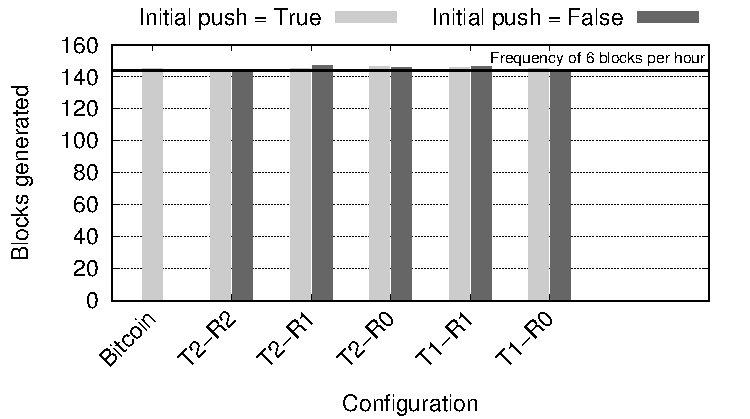
\includegraphics[width=0.7\textwidth]{plots/blocks-gen.pdf}
\caption{Blocks generated.}
\label{fig:nb-blocks}
\end{figure}

\begin{figure}
\centering
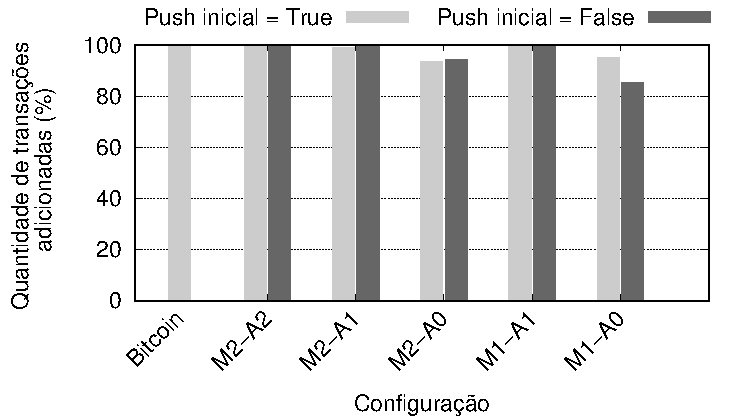
\includegraphics[width=0.7\textwidth]{plots/tx-added.pdf}
\caption{Percentage of transactions committed.}
\label{fig:tx-added}
\end{figure}

Figure~\ref{fig:nb-blocks} shows, for each configuration, the amount of blocks that were generated during each experiment, while Figure~\ref{fig:tx-added} shows the percentage of transactions added to blocks. As it is possible to observe, the simulation generated the expected amount of blocks for a day ($\approx 144$) and committed all the created transactions ($\approx 100\%$). This shows that, for every configuration, all transactions reached at least a miner that added them to a block.

\begin{figure}
\centering
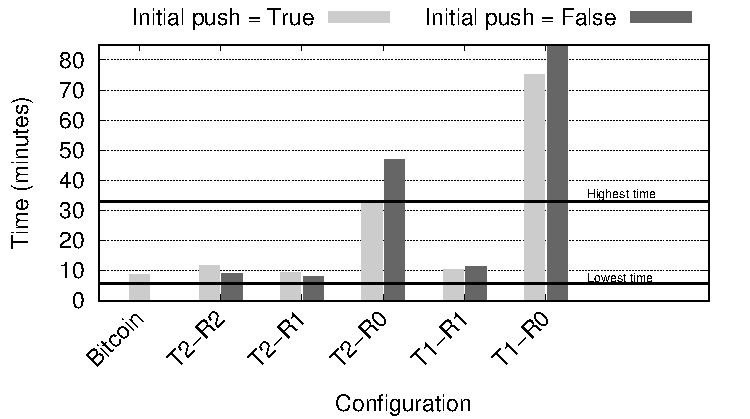
\includegraphics[width=0.7\textwidth]{plots/commit-time.pdf}
\caption{Average time it takes for a transaction to be committed.}
\label{fig:commit-time}
\end{figure}

We also measured the average transaction commit time for each configuration, depicted in Figure~\ref{fig:commit-time}.
%takes for committing a transaction.
The horizontal lines represent the highest and lowest average time it took for a transaction to be committed in Bitcoin. We can clearly see that both configurations \textsl{T2-R0} and \textsl{T1-R0} are not good enough to achieve a commit time comparable to Bitcoin.
%inside the desired spectrum .
This shows that sending transactions for at least one random node alongside the top nodes has a great impact in the commit time as previously discussed in Section~\ref{sec:sr}.

\begin{figure}
\centering
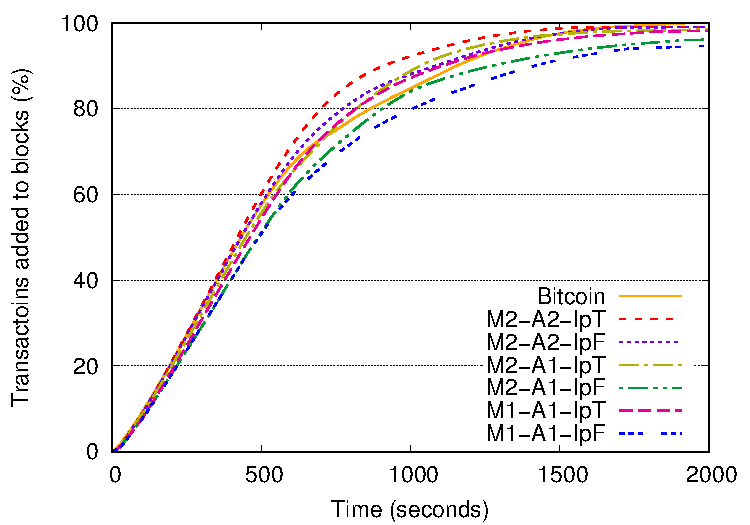
\includegraphics[width=0.7\textwidth]{plots/cdf_commit.pdf}
\caption{Cumulative distributed function of the time it takes for a transaction to be committed.}
\label{fig:cdf-commit}
\end{figure}

Figure~\ref{fig:cdf-commit} shows the cumulative distributed function of the time took to commit all the transactions, hence, it is a different perspective of Figure~\ref{fig:commit-time}. We can  observe sending a new transaction it to all the neighbours (\emph{ip=T}) has a very low impact in the time it takes to commit a transaction.
We attribute this to the fact that the time it takes for a transaction to reach all the miners is orders of magnitude (few seconds versus dozen of minutes) lower than the rate at which blocks are being generated.

With the impact of each configuration in the transaction commit time and number of transactions analysed, we now focus on the impact on reducing network usage.

%Having analysed the impact of our approach in terms of observable effects in the network like how much time it takes for a transaction to be added to a block and amount of transactions committed we will now focus on the savings in terms of messages sent and in the amount of information transmitted.
\begin{figure}
\centering
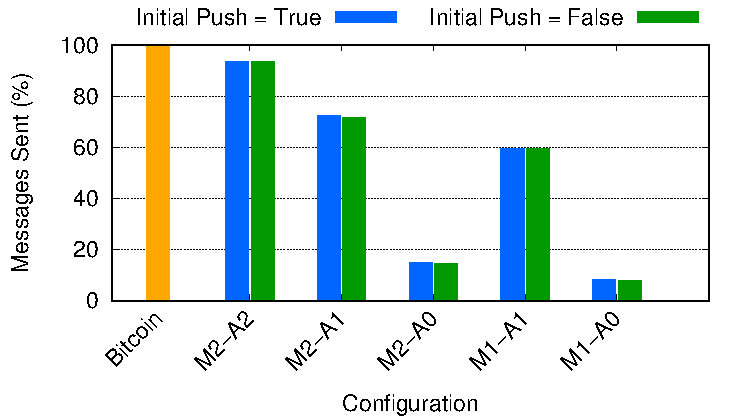
\includegraphics[width=0.7\textwidth]{plots/msg-sent.pdf}
\caption{Total number of messages sent.}
\label{fig:msg-sent}
\end{figure}

\begin{figure}
\centering
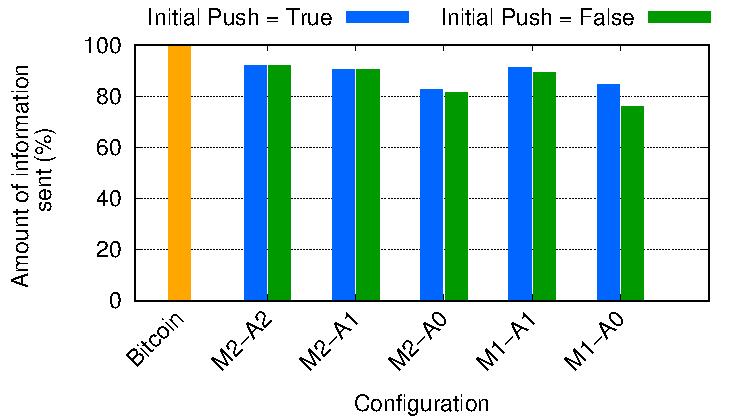
\includegraphics[width=0.7\textwidth]{plots/mb-sent.pdf}
\caption{Amount of information sent.}
\label{fig:mb-sent}
\end{figure}

Figure~\ref{fig:msg-sent} shows ratio between the total number of messages sent in to the same amount in the Bitcoin network. As expected, the configurations with a higher amount of savings were the configurations that did not relay to random nodes. This happens because when we send a transaction to a random node there is a higher chance that that node still does not have that transaction and will request it. Unfortunately, as we have seen previously, both these configurations are not viable because both take very long to commit transactions. Figure~\ref{fig:mb-sent} shows a different perspective by depicting the savings in the total amount of information transmitted which,a s expected, follows a similar pattern to Figure~\ref{fig:msg-sent}. We can also see that the savings from Figure~\ref{fig:mb-sent} are not as big as the ones from Figure~\ref{fig:msg-sent}.
This happens because the advertise messages that we avoid sending are not very big in size. However, processing those spurious incurs an additional cost to the nodes.
%messages in the real worlds always takes a toll on the nodes.

By analysing these results, we can conclude that the most promising configuration is \textsl{T1-R1} with \textsl{ip=False} because not only  it achieves relevant savings (reduction in the number of messages sent in $41.5\%$ and reduction of the amount of information sent in $10.2\%$) but also it preserves the properties of the original Bitcoin.

\subsection{Effect of Adaptation}
To determine the best possible configuration we used a stable network, where miners were always the same nodes. However, as in any large network, Bitcoin is prone to changes.
%, given that is a peer-to-peer network.
We now study the adaption policy introduced in Algorithm~\ref{alg:inc}.
%referenced in Section~\ref{sec:nc}, as well as,
Initially, all nodes send advertisements to all their neighbours as in the regular Bitcoin. Then throughout the simulation, the algorithm will progressively determine the best Tn-Rn configuration for each node. We performed three experiments, one where we did not make any changes to the network, another where we change two miners in the network at 12 hours into the simulation and finally a third one where we changed all the miners at 12 hours into the simulation. With these experiments, we want to determine if our solution is able to adapt to the network changes and preserve the commit time while still sending as few messages as possible.

\begin{figure}
\centering
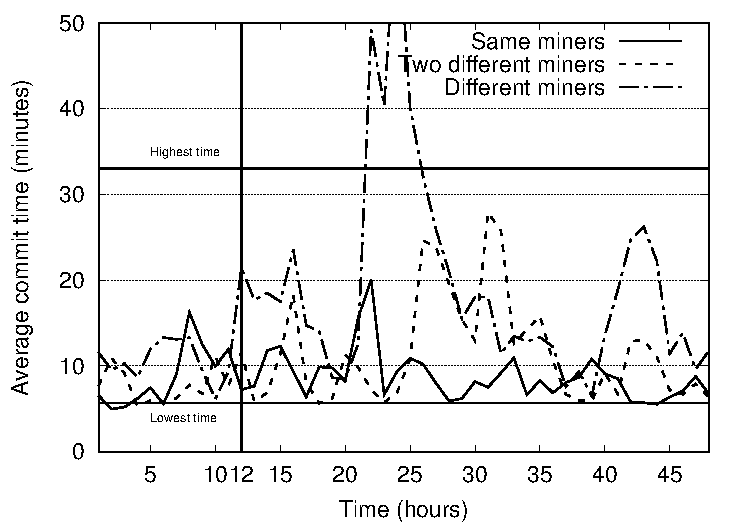
\includegraphics[width=0.7\textwidth]{plots/commit_over_time.pdf}
\caption{Average commit over time.}
\label{fig:commit-over-time}
\end{figure}

\begin{figure}
\centering
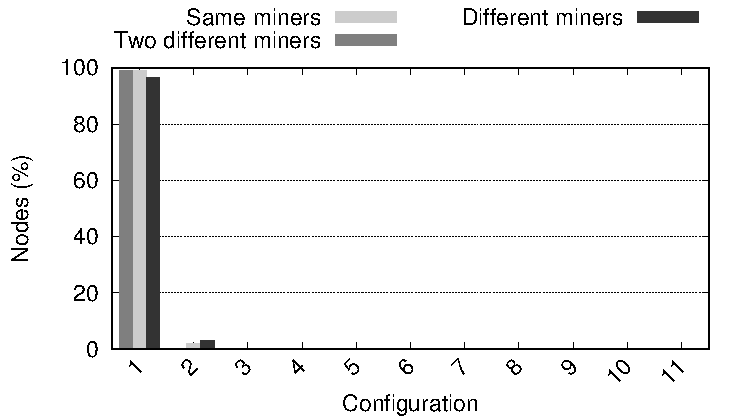
\includegraphics[width=0.7\textwidth]{plots/nodes_per_config.pdf}
\caption{Distribution of the nodes by the different possible configurations.}
\label{fig:node-per-conf}
\end{figure}

Figure~\ref{fig:commit-over-time} shows the average commit time over the period of time simulated. It also shows the two horizontal lines that were in Figure~\ref{fig:commit-time}, delimiting the minimum and maximum observed Bitcoin commit time. Figure~\ref{fig:node-per-conf} displays the percentage of nodes in each configuration at the end of the simulation for the three runs.
We can drawn several interesting configurations.
%From both of these images, we can conclude a couple %of things.
First, we can see that if we are in the presence of a stable network, then our solution is going to start adapting to the network and converge to the configuration that we previously deemed ideal (\textsl{T1-R1}), as seen in Figure~\ref{fig:node-per-conf}. Secondly, we can conclude that if there are slight changes to the network, then the average commit time of our solution is going to deteriorate a little bit, but soon after the algorithm will increase the size of \textsl{T} and \textsl{R} to cope with the changes and the average commit time will once again converge to more regular times. Finally, if our solution is confronted with drastic changes to the network it will not be able to maintain the current commit time, given that at 12 hours into the simulation most nodes were configured to \textsl{T1-R1} which is not resilient enough for these cases.
We note however that such sudden shift in mining power is unlikely to happen.
Regardless, after some time our approach will start converging to the desirable stable configuration.
%However, eventually, our solution will start converging to the desired time.
%Note that in our experiments we configured the most desirable configuration to be the one where we send as few messages as possible (\textsl{T1-R1}) but if for instance, we wanted to maintain the commit time in very dynamic environments then the most desirable configuration would probably be \textsl{T2-R2} as it would be more resilient against dramatic changes.
